\chapter{Structure of language and neural language models}\label{chp:background}


\startcontents[chapters]
\printmyminitoc{
}

This chapter provides the background knowledge necessary for understanding the core discussions of this dissertation. Section~\ref{sec:struc_lang} presents key linguistic assumptions regarding human language structures. Section~\ref{sec:nlms} introduces neural language models, with a special focus on the autoregressive Transformer language model --- the main investigation object of this thesis. Lastly, Section~\ref{sec:review_structure_nlm} offers a review of research methodologies that analyze the representation of linguistic structures in neural NLP models.

\section{Structure in human language} \label{sec:struc_lang}

Human language, in its essence, is a structured system that enables communication and the expression of thoughts and meaning, showcasing our unparalleled cognitive capabilities. Traditional linguistic theories, tracing back to seminal work by Chomsky and his peers, have long argued that the foundation of our linguistic abilities lies in the presence of intricate, innate structures within the human brain~\citep{chomsky1965aspects,chomsky1986knowledge}. 

Central to these theories is the emphasis on the hierarchical nature of language. Rather than viewing sentences as mere strings of words, traditional linguistics posits that sentences have an underlying structure, where larger linguistic structures are recursively built from smaller components. This hierarchical arrangement allows for the nesting of linguistic elements within one another, leading to the creation of complex sentences and intricate meanings. According to this view, humans are born with a Universal Grammar --- a set of fundamental principles that govern the structure of all human languages. The recursive nature of this symbolic system, using finite means (words and rules), enables the generation of an infinite number of expressions, showcasing the remarkable productivity of language~\citep{chomsky1965aspects, hauser2002faculty}.

Linguistics often represents the hierarchical and recursive nature of language using discrete, symbolic representations like categorical labels and tree-like hierarchical structures~\citep{berwick2016only}. Words are categorized based on their roles and functions in sentences, referred to as their grammatical or syntactic categories, commonly known as \ac{PoS} tags in NLP (e.g., \texttt{noun}, \texttt{verb}). This hierarchical organization of words in sentences can be visualized as syntactic trees (Figure~\ref{fig:sent_tree}), where nodes represent syntactic categories (e.g., noun phrases (NP) or \ac{VP}), or individual words. Edges connect these nodes, with their left or right positioning indicating ordered relationships. Through this representation, the tree captures the hierarchical relationships between words and phrases.\footnote{Note that the provided syntactic tree is merely illustrative. In actual linguistic practice, the labels and structures vary according to the specific linguistic formalism being used.} 


\begin{figure}[ht]
    \centering
        \centering
    \begin{forest}
        for tree={s sep=8mm,, inner sep=0, l=0}
        [,phantom,s sep=2.5cm
        [S   
            [NP [Emma]]
            [VP
                [V[saw ] ]
                [NP 
                     [the dog, roof]   
                ]
            ]
        ]
        ]
    \end{forest}
    \caption{Syntactic tree: a hierarchical representation of word organization in sentences} \label{fig:sent_tree}
    \end{figure}
    
\begin{figure}[ht]
    \centering
    \begin{forest}
        for tree={s sep=8mm,, inner sep=0, l=0}
        [,phantom,s sep=2.5cm
        [\small  \texttt{$see'(\text{{Emma}},\iota x.dog'(x))$} 
            [\small Emma [Emma]]
            [\small \texttt{$\lambda b.see'(b,\iota x.dog'(x))$}
                [\small \texttt{$\lambda .a\lambda b.see'(b,a)$}[saw ] ]
                [\small \texttt{$\iota x.dog'(x)$} ,alias=o, 
                     [the dog, roof]   
                ]
            ]
        ]
        ]
    \end{forest}
    \caption{The sentence's meaning is derived compositionally from the meaning of its components, in line with its syntactic structure in Figure~\ref{fig:sent_tree} \label{fig:sent_meaning} }
\end{figure}

Linguists largely agree that the principle of compositionality underpins the productivity of language, with a common focus on semantic compositionality. As articulated by Frege and later expanded by Partee, the principle of compositionality posits that the meaning of a linguistic expression is derived from the meanings of its individual components and their syntactic arrangement~\citep{frege_1892,partee1984compositionality}.  This principle is crucial as it explains our ability to understand and produce a vast array of sentences, even those we have never previously encountered. Using tools from symbolic logic, formal semantics maps syntactic structures --- how words are arranged --- to semantic structures (their associated meanings). This approach allows us to clearly illustrate, as illustrated in Figure~\ref{fig:sent_meaning}, how the meaning of a sentence is derived from the meanings of its constituent parts.

In essence, traditional linguistic theories advocate for a symbolic representation of language. They argue that our linguistic competence does not solely emerge from statistical learning or exposure to language data. Instead, it is rooted in complex, innate structures that guide our understanding and production of language~\citep{chomsky1965aspects, hauser2002faculty}. This perspective has been foundational in shaping our understanding of human language and continues to influence linguistic research and debate.

Traditional NLP models have deep roots in linguistic theory. A typical NLP pipeline incorporates a range of intermediate linguistic modules, each designed to extract specific linguistic knowledge from human-annotated data, such as POS tagging, syntactic parsing, and semantic role labeling. These modules help transform textual information into structured, symbolic forms that can be readily processed and analyzed. Before the rise of deep learning, these symbolic representations served a crucial role in NLP models. They were either directly incorporated into models as input data --- obtained through linguistic feature engineering --- or indirectly learned through models that extract linguistic patterns from corpora annotated by human linguists. Despite their interpretability benefits, these traditional models heavily depend on time-consuming feature engineering and extensive linguistic annotation, which limit their scalability and their capacity to generalize across different languages and domains. Furthermore, given the vast complexity and variability inherent to natural language, these models often struggle to effectively handle language processing based solely on small amounts of manually annotated data.
 

\section{Neural language models}\label{sec:nlms}

Neural language models (NLMs), central to the deep learning tsunami in natural language processing, fundamentally shift the paradigm from manual feature engineering to directly learning language  representations from raw text data~\citep{manning-2015-last}. In this section, we delve into a comprehensive overview of neural language models. Section~\ref{sec:lm_tasks} introduces the concept of language modeling --- the task that enables NLMs to incorporate their understanding of different facets of language into their internal representations. Following this, Section~\ref{sec:auto_transformer} offers an in-depth look at the Transformer-based neural language models, in particular the autoregressive language model, a sub-type of NLMs and the main focus of this dissertation. In this subsection, we outline the Transformer architecture and describe the mathematics and intuitions behind its various components, with a particular focus on the self-attention mechanism.


\subsection{Language modeling} \label{sec:lm_tasks}

For a language denoted as ${\cal L}$, a language model is a probability distribution over ${\cal L}$ such that the sum of probabilities for all possible sentences equals 1. This probability distribution estimates the likelihood of words or word sequences appearing in ${\cal L}$. For example, it could predict that ``The cat on the mat meowed'' is much more likely to appear in a text than ``The cat on the mat shouted''. 

A language model computes the probability of a sequence as the joint probability of each word, which can be decomposed into the product of conditional probabilities using the chain rule of probability:
\vspace{-0.5\baselineskip}
  \begin{align*}
  \mathbb{P} (s) = \mathbb{P}(\text{The cat on the mat meowed}) = \ 
& \mathbb{P}(\text{The}) \cdot  \mathbb{P}(\text{cat | The}) \cdot \mathbb{P}(\text{on | The cat}) \cdot \\
& \mathbb{P}(\text{the | The cat on}) \cdot \mathbb{P}(\text{mat | The cat on the}) \cdot \\
& \mathbb{P}(\text{meowed | The cat on the mat})
\vspace{-0.2\baselineskip}
\end{align*}
\noindent where $\mathbb{P}(\text{meowed | The cat on the mat})$ represents the conditional probability of the word ``meowed'' given the context of the previous words ``The cat on the mat''.  More generally, for a sequence of words $s = w_1, w_2, ..., w_t$, its probability is calculated as: 
\begin{align}
\mathbb{P}(s) = \mathbb{P}(w_1, w_2, ..., w_t) & = \mathbb{P}(w_1) \cdot \mathbb{P}(w_2 | w_1) \cdot \mathbb{P}(w_3 | w_1, w_2) \cdot ... \cdot \mathbb{P}(w_t | w_1, ..., w_{t-1}) \nonumber \\
&=\prod_{i=1}^{t} \mathbb{P}(w_i | w_{1:i-1})
\end{align}
\noindent
In computational linguistics, this conditional probability $\mathbb{P}(w_i|w_1\ldots
  w_{i-1})$ is particularly useful as it allows to predict the next
  word $w_i$ based on its preceding context $w_1\ldots   w_{i-1}$ in the sentence. 

Language modeling involves training language models on large text corpora to approximate the probability distribution of sequences in a language, using the next word prediction task. Through this training process, the model learns statistical patterns and word relationships, enabling it to predict word sequences effectively. This capacity is crucial for various NLP tasks. For example, in text generation, a chatbot can produce contextually relevant and coherent responses by predicting the most probable next words based on the given input. 

\paragraph{N-gram language models} Traditional language models estimate probabilities by counting word and word sequence frequencies in a training corpus. Predicting the next word $w_i$ based on its entire preceding context $w_1, ..., w_{i-1}$ is challenging due to the exponential growth of possible word combinations. Long sequences suffer from the curse of dimensionality, leading to sparse representations. To address this, early models like n-grams introduce the Markov assumption. It simplifies the task by assuming that the probability of a word depends only on the last $n-1$ words, instead of the entire context.
 For instance, in a bigram model (where $n=2$), $w_i$ is assumed to depend only on the previous word $w_{i-1}$. So, instead of computing
$\mathbb{P}(\text{meowed | The cat on the mat})$,
a bigram model approximates it as
$\mathbb{P}(\text{meowed | mat})$.
This estimated probability can then be computed as the count of the bigram $C(w_{i-1}w_i)$ over the sum of all the bigrams starting with $w_{i-1}$ in the training data:
\begin{equation}
\mathbb{P}(w_i | w_{1},...,w_{i-1}) \approx \mathbb{P}(w_i | w_{i-1}) = \frac{C(w_{i-1}w_i)}{\sum_{w}C(w_{i-1}w)}
\end{equation}

\noindent For the general case of an n-gram language model, the estimated probability of the entire $S$ is given by: 
\begin{equation}
    \mathbb{P}(S) = \mathbb{P}(w_1, w_2, ..., w_t) \approx \prod_{i=1}^{t} \mathbb{P}(w_i |w_{i-(n-1)}, ..., w_{i-1})
\end{equation}

N-gram models marked a shift from rule-based to statistical methods, foundational for early speech recognition and machine translation~\citep{jelinek1998statistical,brown-etal-1993-mathematics}. However, they exhibit significant limitations. Most prominently, their parameters increase exponentially with n-gram order and face data sparsity challenges. They cannot
handle unseen n-grams and struggle with long-distance word dependencies due to their fixed context window. 

The limitations of the N-gram model prompted a shift to neural language models, which use artificial neural networks (i.e., learnable functions) for language modeling. Instead of relying solely on word counts, they learn continuous representations, which are high-dimensional vectors (known as word embeddings), for words and their contexts. This allows them to generalize to unseen word sequences. Moreover, they allow for the processing of longer sequences, thus enabling them to consider larger context windows. 

Artificial neural networks (NN) are computational models originally inspired by biological neural networks~\citep{mcculloch1943logical,rosenblatt1958perceptron}. As shown in Figure~\ref{fig:nn_graph}, the basic building block of an NN is the artificial neuron, referred to as a ``node'' or ``unit''. These neurons are grouped into layers: the input layer receives data features, the hidden layers learn patterns, and the output layer produces predictions. Neurons in one layer connect to those in the next through weighted connections. Each neuron processes its input by applying a weighted sum followed by a nonlinear activation function. It then sends this processed output to the subsequent neurons. During training, the weights are adjusted using an error backpropagation algorithm to minimize the difference between the network's output and the actual targets~\citep{rumelhart1985learning}. Mathematically, a neuron's operation is:
\begin{equation}
    y = f\left( \sum_i w_i x_i + b \right)
\end{equation}
\noindent where $x_i$ represents inputs, $w_i$ are weights, $b$ is a bias term, and $f$ is a non-linear activation function like the sigmoid or relu. The power of NNs comes from their ability to approximate almost any function given enough neurons and layers.


 
\begin{figure}[ht]
    \centering
\begin{tikzpicture}[shorten >=1pt,->,draw=black!50, node distance=2.5cm]
\tikzstyle{every pin edge}=[<-,shorten <=1pt]
\tikzstyle{neuron}=[circle,fill=black!25,minimum size=17pt,inner sep=0pt]
\tikzstyle{input neuron}=[neuron, fill=gray!50];
\tikzstyle{output neuron}=[neuron, fill=red!30];
\tikzstyle{hidden neuron}=[neuron, fill=blue!30];
\tikzstyle{annot} = [text width=4em, text centered]
% Draw the input layer nodes
\node[input neuron, pin=left:Input \# 1] (I-1) at (0,-1) {$e_{i-1}$};
% Label above the first neuron
\node[above of=I-1, node distance=1.5cm] {Input layer};

% Draw the second input neuron with label $e_i$
\node[input neuron, pin=left:Input \# 2] (I-2) at (0,-2) {$e_i$};
% Draw the hidden layer nodes
\foreach \name / \y / \content in {1/1/, 2/2/,  3/3/\vdots, 4/4/}
\path[yshift=0.5cm]
node[hidden neuron] (H-\name) at (2.5cm,-\y cm) {$\content$};
% Label above the first neuron
\node[above of=H-1, node distance=1cm] {Hidden layer};

% Draw the output layer node
\foreach \name / \y / \content in {1/1/\hat{y}_1, 2/2/\hat{y}_2, 3/3/\hat{y}_3, 4/4/\vdots, 5/5/\hat{y}_{|V|}}
\path[yshift=0.8cm]
node[output neuron] (O-\name) at (5cm,-\y cm) {$\content$};
\node[above of=O-1, node distance=0.68cm] {Output layer};
\node[below of=H-4, node distance=0.6cm] {$h^i$};

\node[right=0.01cm of O-1] {\small $\mathbb{P}(a|..)$};
\node[right=0.01cm of O-2] {\small $\mathbb{P}(aardvark|..)$};
\node[right=0.01cm of O-3] {\small $\mathbb{P}(aback|..)$};
\node[right=0.01cm of O-5] {\small $\mathbb{P}(zebra|..)$};


% Connect every node in the input layer with every node in the hidden layer.
\foreach \source in {1,...,2}
\foreach \dest in {1,...,4}
\path (I-\source) edge (H-\dest);
% Connect every node in the hidden layer with the output layer
\foreach \source in {1,...,4}
\foreach \dest in {1,...,5}
\path (H-\source) edge (O-\dest);

\draw[->,gray,line width=0.1pt] (I-2) -- node[midway,below,yshift=-0.2cm,text=black] {\large $W_{in}$} (H-4);
\draw[->,gray,line width=0.1pt] (H-4) -- node[midway,below,yshift=-0.2cm,text=black] {\large $W_{out}$} (O-5);
\end{tikzpicture}
    \caption{Forward inference in a feed-forward neural language model with window size of two, at timestep $i+1$. To predict the next word $w_{i+1}$, the model concatenates embeddings of the two preceding words, $\ivec{e}_{i}$ and $\ivec{e}_{i-1}$, multiplies them by $\ivec{W}_{in}$, and applies an activation function to produce the hidden layer. This layer is then transformed by $\ivec{W}_{out}$ and a softmax to estimate the probability of each word in its vocabulary being the next word $w_{i+1}$.}
    \label{fig:nn_graph}
\end{figure}

\vspace{-0.5\baselineskip}
\paragraph{\ac{FFNLM}} The FFNLM applies a feed-forward neural network, a subtype of NN with unidirectional information flow (i.e., without looping back or cycles), for language modeling~\citep{ffnlm_bengio}. Similar to n-gram models, it employs a Markov assumption by considering a fixed number of previous words as context to predict the next word. In this model, words are first transformed into word embeddings. The embeddings from preceding $k$ words are then fed into a feed-forward neural network, which in turn produces a probability distribution over possible next words. For instance, Figure~\ref{fig:nn_graph} illustrates how to predict the next word $w_{i+i}$ in an FFNLM with a context window size of $k=2$. Formally, the defining equations at timestep $i+1$ are:
\begin{align}
      P(w_{i+1}|w_{i-1}w_{i}) &= \textsc{softmax}(\ivec{W}_{out}\ivec{h}^{i}+\ivec{b}_{out}) \nonumber \\
      \ivec{h}^{i} &= g( \ivec{W}_{in}
                 \begin{bmatrix}
                   \ivec{e}_{i}\\
                   \ivec{e}_{i-1}
                   \end{bmatrix}+\ivec{b}_{in})
\end{align}
\noindent where $W_{in} \in \mathbb{R}^{d_h \times 2d}$, $W_{out} \in \mathbb{R}^{|V| \times d_h}$, with $d_h$ denoting the hidden layer size, $d$ the embedding size, $|V|$ the vocabulary size and $g$ refers to the activation function.

However, despite being an advance over n-gram models, FFNLMs still have a fixed context size, which restricts their ability to capture long-range dependencies in text.

\paragraph{RNN language model} \ac{RNN} language models~\citep{elman1990finding,mikolov2010recurrent} overcome the limitations of the Markov assumption through recurrence. Unlike the feed-forward model, an RNN iteratively updates its hidden layers to capture information about the previous steps in the sequence. It processes the text one element at a time, predicting the next word based on the current word and the previous hidden state. Theoretically, this allows the model to retain information from the sentence's start to the present word, eliminating fixed context size constraints. As shown in Figure~\ref{fig:rnn}, while the forward inference of RNN is very similar to that of feed-forward NLM, the key distinction lies in the RNN's capacity to maintain and use a memory of prior timesteps through its hidden states. Formally, the defining equations at timestep $i+1$ are:
\begin{align}
      \mathbb{P}(w_{i+1}|{\color{red} w_{1}}\ldots w_{i}) &=
        \textsc{softmax}(\ivec{W}_{out}\ivec{h}^{i}+\ivec{b}_{out}) \nonumber\\
      \ivec{h}^{i} &= g( \ivec{W}_{in} \ivec{e}_{i} +\ivec{b}_{in} +\ivec{W}_{rec} \ivec{h}^{i-1}   )
\end{align}
\noindent Here, $\ivec{h}^{i}$ is an update of $\ivec{h}^{i-1}$, integrating the information from the current word, $\ivec{e}_{i}$. Essentially, $\ivec{h}^{i}$ can be considered as a vector encoding the information from the starting word $e_1$ up to the current word $e_i$.

\begin{figure}[ht]
\centering
\begin{tikzpicture}[
      neurons/.style 2 args={
        rectangle split,
        rectangle split horizontal,
        draw=#2,
        rectangle split parts=#1,
        fill=#2!20}]

\node[neurons={3}{yellow}] (s1) at (0,2) {};
\node[neurons={3}{yellow}] (s2) at (2,2) {};
 \node[neurons={3}{yellow}] (s3) at (4,2) {};
 \node[neurons={3}{yellow}] (s4) at (6,2) {};
 \node[neurons={3}{red}] (s5) at (8,2) {};
\node (w6) [above=8mm of s5.center] {meows};
      
 \node[neurons={3}{blue}] (h1) at (0,1) {};
 \node[neurons={3}{blue}] (h2) at (2,1) {};
 \node[neurons={3}{blue}] (h3) at (4,1) {};
 \node[neurons={3}{blue}] (h4) at (6,1) {};
 \node[neurons={3}{blue}] (h5) at (8,1) {};

 \node[neurons={3}{black}] (x1) at (0,0) {};
 \node[neurons={3}{black}] (x2) at (2,0) {};
 \node[neurons={3}{black}] (x3) at (4,0) {};
 \node[neurons={3}{black}] (x4) at (6,0) {};
 \node[neurons={3}{black}] (x5) at (8,0) {};

  \node (w7) [left=10mm of x1.center,align=center] {Input \\ embeddings};
  \node (w8) [left=10mm of h1.center,align=center] {hidden layer};
  \node (w9) [left=10mm of s1.center,align=center] {Output layer};

  \node (w1) [below=5mm of x1.center] {A};
 \node (w2) [below=5mm of x2.center] {cat};
 \node (w3) [below=6mm of x3.center] {on};
 \node (w4) [below=5mm of x4.center] {the};
 \node (w5) [below=5mm of x5.center] {mat};
\draw [->,thick] (s5) -- (w6)node[pos=0,right,yshift=7pt] {\textsc{softmax}};

\draw [->,gray] (x1) -- (h1);
\draw [->,gray] (x2) -- (h2);
\draw [->,gray] (x3) -- (h3);
\draw [->,gray] (x4) -- (h4);
\draw [->,thick] (x5) -- (h5)node[pos=0,right,yshift=6pt] { $\ivec{W}_{in}$};


\draw [->,gray] (h1) -- (s1);
\draw [->,gray] (h2) -- (s2);
\draw [->,gray] (h3) -- (s3);
\draw [->,gray] (h4) -- (s4);
\draw [->,thick] (h5) -- (s5)node[pos=0,right,yshift=6pt] { $\ivec{W}_{out}$};

\draw [->,gray] (h1) -- (h2);
\draw [->,gray] (h2) -- (h3);
\draw [->,gray] (h3) -- (h4);
\draw [->,thick] (h4) -- (h5)node[pos=0.5,above,yshift=3pt] {\small $\ivec{W}_{rec}$};
\end{tikzpicture}
\caption{Forward inference in an RNN language model at timestep $i+1$. To predict the next word after the context ``A cat on the mat'', the model takes the embedding of the current word `mat' and multiplies it by $W_{in}$. Concurrently, it multiplies the hidden layer of the previous timestep $h_{i-1}$ by $W_{rec}$. These values are summed and passed through an activation function to produce the current hidden layer, $h^i$, which is then transformed by $\ivec{W}_{out}$ and a softmax to produce a probability distribution over the vocabulary.}\label{fig:rnn}
\end{figure}

RNNs, with their recurrent nature, can capture longer dependencies but face challenges with extended sequences due to the vanishing or exploding gradient issue. The \ac{LSTM} network, an advanced RNN variant, tackles the gradient problems through its sophisticated gated architecture. This structure helps the model decide when to keep or discard information across longer sequences, enhancing its ability to handle long-distance dependencies. Even with these improvements, LSTM still struggles with very long sequences. 
 

\paragraph{Transformer-based language models} Introduced by~\citep{NIPS2017_3f5ee243}, the Transformer architecture has revolutionized NLP. At the heart of the Transformer architecture is the self-attention mechanism, detailed in Subsection~\ref{sec:auto_transformer}, which theoretically allows each word to relate directly with every other word, irrespective of distance. The original model consists of an encoder-decoder structure, where the encoder is trained to convert input sequences into contextualized representations, while the decoder generates task-specific output sequences, using the previous output for context at each step. This design, often referred to as \ac{Seq2Seq}, is intended for Seq2Seq tasks, such as machine translation and text summarization. 

Due to its parallel processing capability and the ability to capture long-range dependencies effectively, the Transformer architecture has been adapted for language modeling~\citep{radford2018gpt1,radford2019language,devlin-etal-2019-bert} and has become the foundation for modern NLMs. Language modeling in Transformer models can be broadly categorized into two types: autoregressive and masked.

Autoregressive Transformer language models, such as the \ac{GPT} series~\citep{radford2018gpt1,radford2019language,brown2020language,openai2023gpt4} and more recent LLaMa~\citep{touvron2023llama}, predict the next word in a sequence based on all preceding words. They typically use only the decoder component of the original Transformer and are widely applied in natural language generation tasks. The main project of this dissertation (\S\ref{chp:main_project}) focuses on a GPT2-like autoregressive Transformer LM, and we test LLaMa in our SLOG project (\S\ref{chp:slog}). 

In contrast, masked Transformer language models such as \ac{BERT}~\citep{devlin-etal-2019-bert}, FlauBERT~\citep{le2019flaubert}, generate token representations by considering both prior and subsequent tokens in a sequence. They are pre-trained using a \textbf{masked language modeling objective},\footnote{Also called ``denoising'' objectives~\citep{taylor1953cloze}} where a certain percentage of input tokens are masked and the model is trained to predict these masked tokens from their surrounding context. These models are typically built using the encoder layers of the original Transformer. While they don't directly model the probability of input sequences as autoregressive models do, making them less suited for generation tasks, they excel at generating contextually rich token representations, widely used in natural language understanding tasks. 

Blending the strengths of both approaches, Seq2Seq language models like T5~\citep{2020t5} frame all NLP tasks as text-to-text problems. During pre-training, various spans of text are masked (similar to BERT), and then the model is trained to predict full sequences autoregressively. This dual nature makes them versatile and suitable for a wide range of NLP tasks, from text generation to classification and translation. We test the structural generalization ability of T5 in Chapter~\ref{chp:slog}.

Transformer-based pre-trained language models have become foundational elements in modern NLP systems due to their ability to learn generic transferable linguistic representations from vast unlabeled text corpora~\citep{kalyan2021ammus}. % and then transfer this knowledge to downstream tasks. 
Such contextualized representations can be used directly as inputs for task-specific text processing models. The transfer-learning paradigm, which includes pre-training followed by various fine-tuning methodologies~\citep{devlin-etal-2019-bert,pruksachatkun2020intermediate,liu2019multi}, further equips these models with task-specific knowledge. More recently, prompt tuning has emerged as an efficient technique that exploits these models to generate context-aware outputs from given prompts~\citep{liu2021pretrain}. Over the past couple of years, Transformer-based language models offer groundbreaking improvements in NLP capabilities, models like GPT-4 can generate coherent human-like text~\citep{bubeck2023sparks}. Moreover, they have inspired architectures in other domains, becoming a cornerstone in the expanding generative AI, which also includes image generation~\citep{ramesh2022hierarchical}, and code generation~\citep{chen2021evaluating}.

On the theoretical front, these contextualized representations have also become a focus of research on language and human language processing~\citeti{baroni2020linguistic,linzen2021syntactic,baroni2022proper,mccoy2018revisiting,liu-etal-2019-linguistic, yedetore-etal-2023-poor}. Researchers have leveraged these representations to investigate how these models process and understand language, what kind of linguistic knowledge they implicitly learn, and how their understanding aligns with or diverges from our knowledge of human language processing. The insights gained from such investigations can help inform both the design of more effective computational models and the theoretical understanding of human language.


\paragraph{Evaluation of language models} Perplexity is a probability-based metric to evaluate the quality of language model on its training task --- predicting next word based on previous words in a sequence. While a language model's performance can always be assessed through improvements in downstream applications, such extrinsic evaluation can be computationally expensive and affected by various task-specific factors. Intrinsic evaluation like perplexity provides a direct and more efficient way to measure the potential improvement of LMs, aiding in model development and comparison.

Formally, for a language model trained on a corpus and tested on a held-out test set, $\mathcal{D}_{t} = w_1, w_2, ..., w_N$, the model's perplexity $PPL$ on this test set is defined as the inverse probability of the test set, normalized by the number of words $N$:
\begin{align}
\mathbb{P}(\mathcal{D}_{t}) &= P(w_1, w_2, ..., w_N)^{-\frac{1}{N}} \nonumber \\
&= \left(\prod_{i=1}^{N} \frac{1}{P(w_i | w_1, \ldots, w_{i-1})}\right)^{\frac{1}{N}}
\end{align}
In practice, working with log probabilities is often preferred as sequence probabilities can become extremely small through multiplication. As language models are typically trained to maximize the log likelihood of the corpus, this definition of perplexity corresponds to exponentiating the average negative log-likelihood:
\begin{equation}
P(W) = 2^{-\frac{1}{N} \sum_{i=1}^{N} \log_2 P(w_i | w_1, \ldots, w_{i-1})}
\end{equation}
Conceptually, perplexity can be viewed as the \textbf{weighted average branching factor} of a language. It represents the average number of plausible
subsequent words that can follow any given word sequence. Thus, the perplexity of a language model on a test set is the average number of equally probable word predictions that the model makes for each actual word in the test set. A lower perplexity score indicates a better language model.  

\subsection{Transformer-based neural language model}\label{sec:auto_transformer}
In the previous section, we have seen that various neural networks can be used for language modeling; in this section, we delve into the Transformer, the current state of the art architecture for language modeling, with a specific focus on the autoregressive variant.

\paragraph{Overview of the Transformer architecture}
Transformer-based models consist of a series of identical Transformer blocks stacked together. As shown in Figure~\ref{fig:transformer_layer}, a standard Transformer block has two main components: a self-attention layer, followed by a fully-connected feed-forward network. Each of these two sub-layers includes a residual connection and is followed by a layer normalization operation.

\begin{figure}[ht]
    \centering
    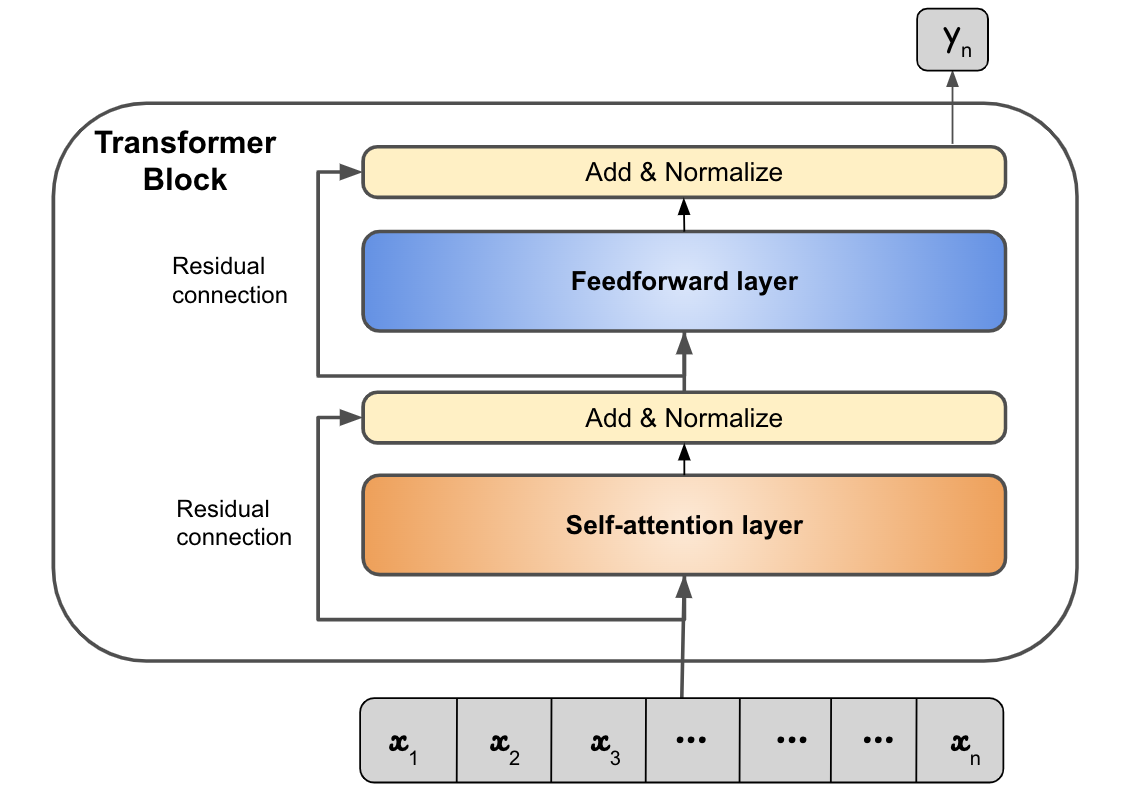
\includegraphics[scale=0.36]{figures/Transformer_layer.png}
    \caption{Components of a typical Transformer block: self-attention, feed-forward network, layer normalization, and residual connections. }
    \label{fig:transformer_layer}
\end{figure}
The self-attention layer, a key innovation of the Transformer architecture, enables the model to focus on different parts of the input when predicting the output for a particular position. This is accomplished by computing a weighted sum of the input sequence, where the weights are determined by the relevance 
of input elements related to the current position.

The feed-forward network (\S\ref{sec:lm_tasks}) applies a position-wise transformation to the attention outputs and allows the model to learn complex patterns. This transformation is the same at each position and includes two linear transformations with a relu activation function in between.

Residual connections play a crucial role in information preservation. These connections allow information from earlier layers to be passed unaltered to later layers, addressing issues such as vanishing gradients~\citep{he2016deep}. Specifically, in Transformer blocks, the output of each sub-layer (self-attention and feed-forward network) is added to its input before being normalized. Layer normalization~\citep{ba2016layer} is applied to these summed vectors to maintain the hidden layer values within an optimal range for gradient-based training. This process involves transforming the inputs to achieve a mean of 0 and a standard deviation of 1 across each layer.


The original Transformer consists of both encoder and decoder stacks, with each stack containing six identical Transformer layers. Early adaptations of Transformer-based models typically stack $l \in \{6, 10,12,16,24\}$ such layers, while the rise of large language models such as GPT-3 has led to architectures with nearly a hundred layers or more~\citep{brown2020language,openai2023gpt4}. In addition to these Transformer blocks, the model includes an input and output embedding layer. The input embedding layer converts each word in the input sequence to a high-dimensional vector, which is then combined with its position encoding to incorporate word order within the sequence. The output layer, on the other hand, is a linear layer followed by a softmax function to produce a probability distribution over the vocabulary for the next word prediction.

A standard formulation of the full Transformer stack is as follows:
\begin{align}
\text{For each layer } l = 1 \text{ to } L:& \nonumber \\
\text{Self-Attention: } & \mathbf{Z}_l^{(1)} = \text{SelfAttn}(\mathbf{Z}_{l-1}) + \mathbf{Z}_{l-1} \nonumber \\
\text{Normalization: } & \mathbf{Z}_l^{(2)} = \text{LayerNorm}(\mathbf{Z}_l^{(1)}) \nonumber \\
\text{Feed Forward: } & \mathbf{Z}_l^{(3)} = \text{FFN}(\mathbf{Z}_l^{(2)}) + \mathbf{Z}_l^{(2)} \nonumber \\
\text{Normalization: } & \mathbf{Z}_l = \text{LayerNorm}(\mathbf{Z}_l^{(3)})
\end{align}
\noindent where $l$ is the layer number, $L$ is the total number of layers, $\mathbf{Z}_l^{(1)}$ is the output of the self-attention mechanism at layer $l$, $\mathbf{Z}_l^{(2)}$ is the normalized self-attention output, $\mathbf{Z}_l^{(3)}$ is the output of the feed-forward network at layer $l$, and $\mathbf{Z}_l$ is the final output of layer $l$ after normalization.

\paragraph{Self-attention mechanism} The core principle behind the attention-based approach is its ability to assess the relevance of different elements within a sequence in relation to a target element. Let's consider an example sentence, ``The cat on the mat ate a fish". As shown in Figure~\ref{fig:self_attention_illu}, while predicting the next word after ``ate", self-attention draws comparisons between the current word ``ate" and all preceding words, including itself. Each pair of words is then assigned a relevance score, which can be calculated as a dot product. 
To compute the final representation for ``ate", the mechanism takes each word's vector representation seen so far, weighs it by the corresponding relevance score, and sums these weighted representations. As a result, words that are more relevant to ``ate" will contribute more to its final representation. 

\begin{figure}[ht]
    \centering 
\scalebox{0.8}{
\begin{tikzpicture}[
      neurons/.style 2 args={
        rectangle split,
        rectangle split horizontal,
        draw=#2,
        rectangle split parts=#1,
        fill=#2!20}]
      
 \node[neurons={3}{green}] (s1) at (0,3) {};
 \node[neurons={3}{green}] (s2) at (2,3) {};
 \node[neurons={3}{green}] (s3) at (4,3) {};
 \node[neurons={3}{green}] (s4) at (6,3) {};
 \node[neurons={3}{green}] (s5) at (8,3) {};
 \node[neurons={3}{green}] (s6) at (10,3) {};
 %\node[neurons={3}{green}] (s7) at (12,3) {};

%\node (o1) [above=5mm of s7.center] {$target$};

 \node[neurons={3}{black}] (x1) at (0,0) {};
 \node[neurons={3}{black}] (x2) at (2,0) {};
 \node[neurons={3}{black}] (x3) at (4,0) {};
 \node[neurons={3}{black}] (x4) at (6,0) {};
 \node[neurons={3}{black}] (x5) at (8,0) {};
 \node[neurons={3}{black}] (x6) at (10,0) {};
 \node[neurons={3}{black}] (x7) at (12,0) {};
 \node[neurons={3}{black}] (x8) at (14,0) {};

  \node (w1) [below=5mm of x1.center] {The};
 \node (w2) [below=5.5mm of x2.center] {cat};
 \node (w3) [below=6mm of x3.center] {on};
 \node (w4) [below=5mm of x4.center] {the};
 \node (w5) [below=5mm of x5.center] {mat};
  \node (w6) [below=5.5mm of x6.center] {ate};
 \node (w7) [below=6mm of x7.center] {a};
 \node (w8) [below=5mm of x8.center] {fish};

\draw [->, color=gray!40] (x1) -- (s1);


\draw [->,color=gray!40] (x1) -- (s2);
\draw [->,color=gray!40] (x2) -- (s2);


\draw [->,color=gray!40] (x1) -- (s3);
\draw [->,color=gray!40] (x2) -- (s3);
\draw [->,color=gray!40] (x3) -- (s3);

\draw [->,color=gray!40] (x1) -- (s4);
\draw [->,color=gray!40] (x2) -- (s4);
\draw [->,color=gray!40] (x3) -- (s4);
\draw [->,color=gray!40] (x4) -- (s4);

\draw [->,color=gray!40] (x1) -- (s5);
\draw [->,color=gray!40] (x2) -- (s5);
\draw [->,color=gray!40] (x3) -- (s5);
\draw [->,color=gray!40] (x4) -- (s5);
\draw [->,color=gray!40] (x5) -- (s5);

%\draw [->,color=gray!40] (x1) -- (s6);
%\draw [->,color=gray!40] (x2) -- (s6);
%\draw [->,color=gray!40] (x3) -- (s6);
%\draw [->,color=gray!40] (x4) -- (s6);
%\draw [->,color=gray!40] (x5) -- (s6);
%\draw [->,color=gray!40] (x6) -- (s6);

\draw [->,ultra thick] (x1) -- (s6);
\draw [->,ultra thick] (x2) -- (s6);
\draw [->,ultra thick] (x3) -- (s6);
\draw [->,ultra thick] (x4) -- (s6);
\draw [->,ultra thick] (x5) -- (s6);
\draw [->,ultra thick] (x6) -- (s6);
%\draw [->,ultra thick] (x7) -- (s7);
\end{tikzpicture}
}
\caption{Masked self-attention in autoregressive Transformer language models: each token is processed considering all the preceding tokens and itself, future tokens are excluded.}
    \label{fig:self_attention_illu}
\end{figure}

Transformers introduce a more sophisticated way of representing how each word contributes to the understanding of other words within a sequence. The attention process discerns three distinct roles: the \textbf{query} (Q), the \textbf{key} (K), and the \textbf{value} (V). The query corresponds to the current focus of attention, the key represents the preceding input item being compared to the attention focus, and the value is employed to compute the output for the current position. To capture these three roles, the self-attention mechanism uses three weight matrices $\ivec{W}^q$, $\ivec{W}^k$, $\ivec{W}^v$, which are learned during the training. They transform each input vector to represent its specific role as a query, key, or value. Given these projections, the score between a current word $x_i$, and a token in the preceding context, $x_j$, is computed as the dot product of their respective \textbf{query} and \textbf{key} vectors --- $q_i \cdot k_j$. To achieve more stable gradients, this score is normalized by dividing it by the square root of the key vectors' dimension. Given a query and the set of keys, \{ $k_1,k_2,...,k_i$ \}, these individual scores are then passed through a softmax function to obtain the attention distribution:   

\begin{equation}
\alpha_1\ldots \alpha_i = \textsc{softmax} \left ( \frac{q_i \cdot k_1}{\sqrt{d_k}},\ldots,\frac{q_i \cdot k_i}{\sqrt{d_k}} \right ) 
\end{equation}
 
\noindent This attention distribution is then used to weigh the respective \textbf{value} vectors of the tokens. The result is a weighted sum of all the \textbf{value} vectors, which serves as the output of the self-attention mechanism for the token under consideration. This process is formally expressed as:

\begin{equation}
y_i = \sum_{j \leq i}{\alpha_{j} \cdot V_j}
\end{equation}

\noindent Since each output $y_i$ is computed independently, this entire attention process can be parallelized using matrix multiplication by considering all the $N$ tokens of the input sequence as a single matrix $X \in \mathbb{R}^{N \times d}$. The entire self-attention process for a sequence of $N$ tokens is computed as:

\begin{equation}
\text{SelfAttention}\left(\ivec{Q},\ivec{K},\ivec{V}\right) = \textsc{softmax} \left (\frac{\ivec{Q} \cdot \ivec{K}^T}{\sqrt{d_k}} \right ) \ivec{V}
\end{equation}

Masked Transformer LMs directly use this self-attention computation. However, the autoregressive Transformer has to maintain the autoregressive property, where a token's prediction relies only on preceding tokens and not future ones. To achieve this, a causal attention mask is applied. The causal mask matrix is formally defined as:
\begin{equation}
\textsc{mask}_{ij} = \begin{cases}
-\infty & \text{if } j > i \\
 0 & \text{otherwise}
\end{cases}
\end{equation}
\noindent Here, the upper triangle (future positions related to the current token), is filled with negative infinity and the lower triangle has zeros. Incorporating this causal mask, the output of a single self-attention layer becomes:
\begin{equation}
\text{SelfAttention}\left(\ivec{Q},\ivec{K},\ivec{V}\right) = \textsc{softmax} \left (\frac{\ivec{Q} \cdot \ivec{K}^T}{\sqrt{d_k}} + \textsc{mask} \right ) \ivec{V}
\end{equation}
\noindent Here, adding a very large negative number (from the mask) to the future positions, ensures that when the softmax function is applied in the next step, these positions will have an attention score of nearly 0. This forces the self-attention mechanism to attend only to its previous words and itself, thereby preventing information flow from any future words. This causal attention mask, as suggested by ~\cite{haviv-etal-2022-transformer} may implicitly introduce positional information into the self-attention layer.


Words within a sentence are interconnected in multiple ways. Consider the sentence ``The cat on the mat ate a fish", the verb ``ate" has a subject-verb syntactic dependency with ``cat" and also shares a semantic relationship, where ``cat" is the agent of the action. %, not the ``mat". 
To capture these different aspects of the syntactic, semantic, and even discourse relationships simultaneously, the Transformer employs multi-head attention. Specifically, each of the $h$ attention heads in a self-attention layer uses its unique learned set of weight matrices: $\ivec{W}_h^K$,$\ivec{W}_h^Q$ and $\ivec{W}_h^V$, to determine the respective \textbf{query}, \textbf{key}, and \textbf{value} vectors. Consequently, the output of the multi-head layer with $h$ heads consists of $h$ distinct vectors, each representing a different facet of the token's contextual relationships. For instance, one head might focus on learning grammatical structures, while another might specialize in capturing thematic relationships. These head-specific outputs are then concatenated and linearly transformed via $\ivec{W}^O$, to produce the final output for each token.

In mathematical terms, for an attention head $i$, the output, $\textsc{head}_i$, for a given sequence of N tokens, $X \in \mathbb{R}^{N \times d}$, is computed as follows:
\begin{align}
\textsc{head}_i = \text{SelfAttention}\left(\ivec{Q},\ivec{K},\ivec{V}\right) \nonumber \\
\ivec{Q} = \ivec{X}\ivec{W_i^Q}; \ivec{K} = \ivec{X}\ivec{W_i^K};\ivec{V} = \ivec{X}\ivec{W_i^V} 
\end{align}
where $\ivec{W_i^Q} \in \mathbb{R}^{d \times d_k}, \ivec{W_i^K} \in \mathbb{R}^{d \times d_k},\ivec{W_i^V} \in \mathbb{R}^{d \times d_v}$ with $d$ denoting the dimensionality of both the input to and output from the model, $d_k$ for the key and query embedding dimensions and $d_v$ for the value embedding dimension. Outputs from each head are concatenated and linearly transformed, producing the final output of a multi-head attention layer: 
\begin{equation}
    \text{MultiHeadAttention}\left(X\right) = \left(\textsc{head}_1 \oplus \textsc{head}_2,...,\oplus \textsc{head}_h \right) \ivec{W}^O
\end{equation}

\noindent where $\ivec{W}^O \in \mathbb{R}^{hd_v \times d}$, and $h$ is the total number of attention heads, $\oplus$ denotes the concatenation operation.


\paragraph{Position embeddings} Unlike RNN, which inherently handles word order information by processing input sequences one element at a time, the Transformer architecture is inherently agnostic to the order of tokens by considering all tokens in the input sequence simultaneously. However, the order of words is crucial to the semantics and syntax of a sequence and is often crucial in many tasks, such as language modeling and sequence-to-sequence translation. To overcome this limitation and inject some sense of position or order into the model, position embeddings were introduced.

One straightforward solution is to directly add positional embeddings to the input embeddings. Just as the model learns an embedding for a word like ``cat'', it can also learn a specific embedding for its position in a sequence such as ``The cat on the mat'', identifying it as the second word. In the original Transformer architecture, positional embeddings are generated using fixed sinusoidal functions. These functions convert integer positions into real-valued vectors, creating a unique positional embedding for each position. Specifically, each dimension of the positional embedding receives a value from a sine or cosine function of a different frequency. Formally, for position $p$ and dimension $i$, the values are defined as:
\begin{align}
    PE_{(p,2i)} &= \sin\left(\frac{p}{10000^{\frac{2i}{d}}}\right) \nonumber \\
    PE_{(p,2i+1)} &= \cos\left(\frac{p}{10000^{\frac{2i}{d}}}\right)
\end{align} %_{\text{model}} distance or difference
where $d$ is the dimension of the embeddings.  These fixed positional embeddings are then added to the standard word embeddings, giving the model a sense of each token's position in the sequence. This position encoding scheme has been extended to learned instead of fixed positional embedding in subsequent models such as BERT~\citep{devlin-etal-2019-bert}, Reformer~\citep{kitaev2020reformer}, RoBERTa~\citep{liu2019roberta}, etc. 

While absolute position embeddings provide a sense of sequence order, they don't directly capture the relative distances between tokens. For instance, by modifying ``the cat ate a fish'' to ``Yesterday, the cat ate a fish'', the absolute positions change but not the core meaning. What matters for meaning is the relative position between ``cat'' and ``fish'', regardless of their absolute position in the sequence. To better capture such relational dynamics, relative position embeddings are introduced~\citep{shaw-etal-2018-self,dai-etal-2019-transformer}. These embeddings shift the focus from the absolute position of a token in a sequence to the relative distances or positional differences between pairs of tokens.


Numerous subsequent models have proposed alternative position encoding schemes. For instance, some approaches integrate position information into the attention matrix instead of the input~\citep{dai-etal-2019-transformer,2020t5}. Others represent positions structurally based on the distances on a sentence's parse tree representation~\citep{wang-etal-2019-self,shiv2019novel}. Improving position representations is an ongoing research focus. The study by \cite{dufter-etal-2022-position} provides a comprehensive review of position encoding within the Transformer architecture.


\section{Analysis of linguistic structure in neural NLP models}\label{sec:review_structure_nlm}

The study of linguistic structures in computational models has a long history, dating back to the work of~\cite{elman1990finding,elman89representation} and~\cite{tabor1994syntactic}. Their pioneering research provided early evidence of the potential for neural networks to learn and embody abstract syntactic structures from non-annotated language data. Transitioning from these early insights to the modern era, the scale and complexity of current models like Transformers have significantly increased. As discussed in previous section, they generate output in the form of complex probability distributions over a large vocabulary of words or sub-words. This, in combination with their high-dimensional representation for inputs and millions of parameterized weights for operations, makes the interpretation of these models challenging.

In recent years, a myriad of analysis methods have been developed to better understand the inner mechanics of NLMs. Many studies suggest that these models have learned a substantial amount of syntactic knowledge that resembles human understanding, while others question the degree to which these models develop abstract structural representations of language. Although recent large language models demonstrate an apparently human-like ability to generate fluent and grammatically correct text~\citep{bubeck2023sparks}, there is yet no consensus on whether these Transformer-based models truly understand and incorporate the linguistic structure.

In this section, we will explore three core methods for interpreting and analyzing the representation of linguistic structure in neural NLP models and also discuss their associated limitations.

\subsection{Challenge sets} \label{sec:behav_test}
Challenge sets, also known as test suites, have a long-standing tradition in NLP, tracing back to work like~\cite{lehmann-etal-1996-tsnlp}. These carefully curated sets include a wide range of linguistic phenomena, often targeting specific syntactic, semantic, or pragmatic properties~\citeti{king-falkedal-1990-using,sennrich-2017-grammatical,isabelle-etal-2017-challenge,naik-etal-2018-stress}. While they were initially employed primarily for evaluating machine translation systems, the evolution and success of neural language models have broadened their application. Largely inspired by the experimental paradigms in psycholinguistics, challenge sets have become one of the important methodologies for investigating the fine-grained linguistic knowledge embodied within NLMs. This approach attempts to answer questions like: How well do neural language models capture linguistic principles, and to what extent do they exhibit human-like grammatical competence?


In psycholinguistics literature, a paradigmatic test for human syntactic capacity comes from agreement phenomena~\citep{bockRegulatingMentalEnergy1992, BOCK199145, bockAttractionsVerbAgreement2001}. For instance, subject-verb agreement in English as illustrated in (\ref{ex:na_en_s-v}): the form of the verb ``are'' is determined by its syntactic subject ``keys'', irrespective of the linear distance between them or the presence of the intervening noun, ``cabinet'', which carries a different grammatical number than the subject, and is often referred to as agreement \textit{attractor}~\citep{BOCK199145}. Such long-distance agreement phenomenon exemplifies the hierarchical organization of language rather than a simple linear structure~\citep{everaert2015}.

\setcounter{exx}{0} % Start numbering examples from 1
\begin{exe}
   \ex\label{ex:na_en_s-v}
The old rusty \textbf{keys} to the cabinet \textbf{are} on the table.
\end{exe}

\cite{linzen-etal-2016-assessing} pioneered the use of subject-verb agreement to assess the syntactic sensitivity of modern NLM. They collected 1.35 million English sentences with present-tense verbs from an auto-parsed Wikipedia corpus and annotated each with the main verb's grammatical number. The model's syntactic ability was then evaluated through a \ac{NA} prediction task. In this task, an LSTM took as input the sentence prefixes like the one in (\ref{ex:sent_prefix}), and was trained to predict the grammatical number of the subsequent verb, either \textit{Singular} or \textit{Plural}.

\vspace{-0.5\baselineskip}
\begin{exe}
   \ex\label{ex:sent_prefix}
The old rusty keys to the cabinet \underline{\ \ \ }
\end{exe}
\vspace{-0.5\baselineskip} 
Linzen and colleagues tested an LSTM with 50 hidden units and found that the model demonstrated near perfect overall accuracy on unseen sentence prefixes. Even in the most challenging cases with four attractors like  (\ref{ex:4_attr})\footnote{Agreement attractors are highlighted with an underline. The subject and target verb are marked in bold.}, the accuracy of the number prediction was still 82\%. 
\vspace{-0.5\baselineskip}
\begin{exe}
   \ex\label{ex:4_attr}
Yet the \textbf{ratio} of \underline{men} who survive to the \underline{women} and \underline{children} who survive in these \underline{events} \textbf{is} not clear. 
\end{exe}
\vspace{-0.5\baselineskip}
From these results, the authors concluded that LSTM models, when provided with explicit supervision, can capture significant grammatical structures, enabling them to reasonably approximate structure-sensitive dependencies.

Building on this experimental approach, \cite{gulordava-etal-2018-colorless} further showed that such long-distance agreement is learnable for an LSTM trained on language modeling (i.e., without explicit supervision). Subsequent research has delved deeper into understanding the capability of NLMs to abstractly represent sentence structures during agreement resolution. This exploration spans various dimensions: different languages~\citep{ravfogel-etal-2018-lstm,gulordava-etal-2018-colorless,lakretz2021mechanisms}, diverse models \citep{bernardy-lappin-2017-using,goldberg19assessing}, and potential confounding factors such as lexical co-occurrences~\citep{gulordava-etal-2018-colorless,lasri-etal-2022-bert} or surface-level heuristics \citep{kuncoro2018perils}. Our research contributes to this body of work, with a focus on French agreement phenomena and autoregressive Transformer LM~\citep{li-etal-2021-transformers}. The majority of these studies converge on the positive finding that neural language models are capable of learning a considerable amount of non-trivial structure information from the (unannotated) training data. More detailed discussions on related work that approaches long-distance agreement tasks can be found in Chapter~\ref{chp:NA_tasks}.

Another significant line of research has sought to expand this experimental approach beyond agreement phenomena to encompass a wider array of syntactic phenomena, such as anaphora, licensing, argument structure alternation, and filler-gap dependencies~\citeti{marvin-linzen-2018-targeted,kann-etal-2019-verb,warstadt-etal-2019-neural,wilcox-etal-2018-rnn,hu-etal-2020-systematic}. These studies typically create precisely drafted templates to generate challenge sets featuring specific linguistic phenomena, and then evaluate a neural network's grammaticality judgement on minimally differing sentence pairs based on grammaticality. Evaluations are conducted either through binary acceptability classification, similar to the number agreement prediction task proposed by~\cite{linzen-etal-2016-assessing}, or by comparing the probabilities that a language model assigns to whole sentences. More recently, \cite{warstadt-etal-2020-blimp} introduced BLiMP, a benchmark of linguistic minimal pairs covering a wide range of English grammatical phenomena. Generally, in these studies, NLMs' performance varies significantly across linguistic phenomena. While the models demonstrate robust knowledge of some syntactic phenomena, such as local subject-verb agreement, ellipsis, and control/raising, they struggle with more subtle semantic and complex syntactic phenomena, including licensing and extraction islands.


\paragraph{Formal languages} Analyzing NLMs' ability to handle linguistic structures is complex due to the intertwining of syntactic, semantic, and statistical regularities in human languages. To precisely focus on syntax-processing, researchers also employ formal languages in challenge sets. Typically, a study using formal languages designs a formal grammar to generate a corpus of sentences. A language model (\S\ref{sec:nlms}) is then trained on this corpus, and the evaluation focuses on the model's capability to recognize sequences from the training set and to generalize these learnings to unseen sequences.

Some studies focus on formal languages that correspond to specific classes in the Chomsky hierarchy, investigating which language classes can be theoretically or empirically learned by NLMs. Early studies have shown that certain regular~\citep{giles1992learning} and context-free~\citep{elman89representation} languages can be learned by different RNN models. Subsequent research found that, with proper parametrization, LSTM networks could learn context-sensitive languages, such as $a^nb^nc^n$, and generalize to longer sequences~\citep{gers2001lstm,weiss2018practical,suzgun-etal-2019-lstm}. In contrast, Transformer models have demonstrated, in theoretical studies, more limited capacities compared to LSTMs when handling regular languages and context-free languages~\citep{bhattamishra-etal-2020-ability,hahn:2020}. However, empirical findings like~\citep{ebrahimi-etal-2020-self} have shown that Transformers can
learn $Dyck_k$ languages from finite samples, matching the performance of LSTMs. 
% yao-etal-2021-self

Others craft formal grammars that mirror specific structures present in natural language. For instance, \cite{lakretz2021can} used a \ac{PCFG} to investigate RNN's ability to handle recursively nested subject-verb agreements, \cite{hupkes2020compositionality} used a set of PCFGs to assess NLMs' capacity in processing hierarchical compositional structure. Notably, \cite{sennhauser-berwick-2018-evaluating} evaluated LSTMs using bracket prediction tasks as a measure of understanding linguistic hierarchical structures.  While their findings confirmed that LSTMs can learn context-free grammar, they also observed that models' good performance stemmed more from efficiently handling nuisance variables rather than truly learning the underlying context-free rules. ~\cite{hahn:2020} has theoretically demonstrated that Transformer-based models struggle with bracket closing and iterated negation tasks, both computations are
considered to be essential to hierarchical structure.

\paragraph{Limitations} Challenge sets shed light on models' fine-grained linguistic capabilities by assessing their responses to specific inputs. However, this approach offers limited insight into the internal representations that the model has learned. Confounding factors, such as the inability to distinguish genuine syntactic comprehension from superficial pattern recognition like frequency-based heuristics, can make their results hard to interpret. To get a more comprehensive picture of NLMs' syntactic abilities, these tests should be supplemented with other methods, such as probing tasks or interpretability techniques that can provide insights into the models' internal workings.



\subsection{Probing classifiers} \label{sec:probing}
%probing tasks~\citep{conneau-etal-2018-cram}, 
 The probing classifier approach, also known as auxiliary prediction tasks~\citep{adi2016fine}, diagnostic classifiers~\citep{veldhoen2016diagnostic}, or linguistic probes~\citep{zhu-rudzicz-2020-information}, 
 is widely used to analyze the linguistic capabilities of neural NLP models. At its core, this approach involves training a classifier --- a ``probe'' --- on a model's internal representation to predict specific linguistic properties. Success in this prediction indicates that the model has encoded the relevant linguistic features. The basic premise is that if a model captures a particular linguistic property, this information should be extractable from its internal representation~\citep{hupkes2018visualisation}. This approach thus seeks to address the question: What linguistic properties are encoded in a model's internal representations, and where are they located within the model?

Formally, we define a model under investigation as a function, $\textsc{NN}:x \leadsto r$, that generates a representation, $r$, for an input element. A probing dataset, denoted as $\mathcal{D} = \{r^{(i)}, z^{(i)}\}$, pairs each representation with its associated linguistic property. The probing classifier can then be defined as a function $\mathcal{C}$ that maps the model's representation to a linguistic property of interest: 
\begin{equation}
    \mathcal{C}: r \leadsto z
\end{equation}

In an early application of this approach, \cite{shi-etal-2016-string} probed the syntactic information in neural machine translation. They extracted the hidden states of an RNN encoder and used them to train a logistic regression classifier, predicting labels related to morpho-syntax, such as PoS tags, constituent labels (e.g., NP, VP), voice, and tense. Their results, showing high probing accuracy relative to baseline measures, led them to conclude that the RNN captures significant syntactic information at both the word and sentence levels. Furthermore, they used probing classifiers to identify where syntactic information was stored across layers, observing that local features were often encoded in lower layers, while more abstract, global information was found in upper layers.

This probing methodology has since expanded to investigate other syntactic facets in RNN models, such as surface sentence structure~\citep{adi2016fine},\footnote{Surface sentence structure refers to sentence length, word identities and word order in ~\cite{adi2016fine}.} parse tree depth~\citep{conneau-etal-2018-cram}, syntactic agreement~\citep{giulianelli-etal-2018-hood} and even semantic properties~\citep{ettinger-etal-2016-probing}. This methodology has also been extensively applied to Transformer-based models~\citeti{tenney2019you,liu-etal-2019-linguistic,jawahar-etal-2019-bert,klafka-ettinger-2020-spying}. Collectively, these investigations have yielded promising results, consistently indicating that neural NLP models trained on vast data do encode a wide array of linguistic properties within their internal representations. An interesting extension of this methodology is the structural probe introduced by~\cite{hewitt-manning-2019-structural}. This probe, distinct yet related to the probing classifier, identified a linear transformation that could extract syntactic parse tree structures from word representation spaces in models like ELMo and BERT, but not from simpler baseline representations. (See Table~\ref{tab:probing_papers} for a categorization of representative work using the probing classifiers.)
%,manning2020emergent
\begin{table}[ht]
    \centering
    \scalebox{0.85}{  \begin{tabular}{p{0.22\textwidth}p{0.18\textwidth}p{0.18\textwidth}p{0.22\textwidth}p{0.18\textwidth}}
        \toprule
        \makecell[l]{Linguistic \\ properties} & \makecell[l]{Probing \\classifiers} & Probed models & Baseline models & Papers \\
        \midrule
        \makecell[l]{PoS, tense,voice, \\constituents} & \makecell[l]{Logistic\\ regression} & LSTM encoder & Phrase/syntax-based system & \cite{shi-etal-2016-string} \\
        \midrule
        \makecell[l]{Surface sentence \\ structure} & MLP &LSTM encoder & CBOW &\cite{adi2016fine}\\
        \midrule
        \makecell[l]{Surface structure,\\ parse tree depth,\\ top constituents} & MLP & \makecell[l]{BiLSTM, \\ConvNet }& Unigram, Human&\cite{conneau-etal-2018-cram} \\
         \midrule
        Syntactic agreement & Linear &LSTM LM& --&\cite{giulianelli-etal-2018-hood}\\
         \midrule
        \makecell[l]{PoS, \\dependency edge}&Linear \&MLP&ELMo&Control tasks&\cite{hewitt-liang-2019-designing}\\
        \midrule
        \makecell[l]{8 core NLP \\ labeling tasks} &MLP& \makecell[l]{CoVe, ELMo,\\GPT, BERT} &\makecell[l]{Lexical baselines,\\randomized ELMo,\\word-level CNN}&\cite{tenney2019you}\\
        \midrule
        Entire parse tree&Linear&ELMo, BERT& \makecell[l]{Non-contextual\\ models}&\cite{hewitt-manning-2019-structural}\\
        \bottomrule
    \end{tabular} }
    \caption{A categorization of some representative studies using probing classifiers to investigate syntactic structures in NLMs, according to linguistic properties examined, classifier types, probed models, and baseline models.}
    \label{tab:probing_papers}
\end{table}

On the other hand, recent studies also highlight potential pitfalls in the probing classifier approach, emphasizing that learned properties should be interpreted in comparison to control baselines. This can be achieved through techniques such as training probes on randomized representations~\citep{conneau-etal-2018-cram,tenney2019you}, using control functions~\citep{hall-maudslay-etal-2020-tale}, or implementing control tasks~\citep{hewitt-liang-2019-designing,ravichander-etal-2021-probing}. Specifically, control tasks are designed in a way that they can only be solved if the probe memorizes the task. Based on this, \cite{hewitt-liang-2019-designing} introduced the concept of \textit{selectivity}, which is defined as the performance gap between a probing task and its control counterpart. Using this metric to guide probe selection, they found that, while linear probes are highly selective, nonlinear probes are generally less so. The effectiveness of such probes with respect to its complexity remains a topic of discussion~\citep{hall-maudslay-etal-2020-tale,ravichander-etal-2021-probing},~\cite{belinkov-2022-probing} provides a comprehensive review on probing methods. 


\paragraph{Limitations} A main limitation of probing classifiers is that they only reveal correlations between linguistic properties and a network's inner representations, but do not necessarily indicate causality. Since these probes operate independently from the model's original task, they do not provide any insight on whether the information discovered by the probe influences the model's predictions. Only a few studies we have seen so far, like the one by~\cite{giulianelli-etal-2018-hood}, address this limitation; we will further explore and categorize such efforts in the following subsection, focusing on the causal analysis approach.


\subsection{Causal intervention analysis} \label{sec:sota_causal_approaches}

While linguistic probes are instrumental in revealing what linguistic properties might be encoded within neural models, they often fail to establish a causal relationship between these properties and the probed model's prediction. Causal intervention analysis fills this gap: it assesses the direct influence of specific model components on predictions by manipulating parts of the model and tracking resultant output changes. In this way, we can answer the causal question: which information is actually being used by neural models? Causal analysis is commonly paired with behavioral tests or probing tasks, providing a comprehensive framework for both uncovering and validating the model's linguistic behaviors.

Causal interventions in neural models vary based on where they are applied within the model. Broadly, these interventions can be grouped into three categories: 
\begin{itemize}
    \item Input-level interventions~\citep{zmigrod-etal-2019-counterfactual,vig2020causal,amini2023naturalistic}
    \item layer-level interventions~\citeti{giulianelli-etal-2018-hood,elazar2021amnesic,vig2020causal,ravfogel-etal-2021-counterfactual,feder-etal-2021-causalm}
    \item neuron unit-level interventions~\citep{bau2018identifying,lakretz-etal-2019-emergence,vig2020causal,mueller-etal-2022-causal}
\end{itemize}

In one of the pioneering works, \cite{giulianelli-etal-2018-hood} combined causal intervention with probing classifiers to explore an NLM's syntactic capabilities. They showed that by intervening on an NLM's internal representations --- guided by the gradients from a probing classifier targeting the subject's plurality --- the model's predictions in the subject-verb agreement task could be altered. Thus, the authors concluded that probing classifiers can identify features that are actually used by the model. Later, the study by \cite{elazar2021amnesic} presents a nuanced view. They explored the effects of erasing specific linguistic information from BERT's representation layers on language modeling. Using the iterative null space projection method (INLP; \cite{ravfogel-etal-2020-null}), they systematically erased linguistic information, such as Part-of-Speech and syntactic dependencies, from BERT's internal representations. The INLP process involves training (linear) probing classifiers to detect these linguistic properties and iteratively erasing the associated features until the representations are no longer predictive of the target property. When comparing the language modeling performance before and after such interventions, they observed that the removal of certain properties, such as phrase boundaries, which had high probing performance, didn't significantly impact language modeling performance. This led them to a conclusion contrasting with \cite{giulianelli-etal-2018-hood}: probing classifiers may not always detect information that the model actively uses for its predictions. 

Further expanding the scope, \cite{vig2020causal} explored gender bias in pre-trained Transformer LMs through a comprehensive causal intervention analysis. They manipulated the grammatical gender in the input, attention weights, and individual neurons to measure their causal impacts on the model's behavior. They found that gender bias predominantly resides in a small part of the network and this bias can be traced back to both direct input influences and indirect pathways via individual neurons and attention heads. The implications of this study extend beyond gender bias, offering a structural-behavioral framework for broader research aimed at interpreting and understanding the inner workings of neural NLP models.  

\paragraph{Limitations} Causal intervention analysis presents a unique perspective for establishing causality in interpreting deep NLP models, thus addressing certain limitations of challenge tests and probing classifiers. However, its implementation can be computationally expensive, especially in complex scenarios like neural-level interventions, and establishing clear cause-and-effect relationships within expansive networks is intricate. These complexities limit its practical application, particularly with state-of-the-art models.

